\section{Introduction}

\subsection*{Background}
The \emph{parallel chip-firing game}, also known as the \emph{discrete
  fixed-energy sandpile model}, is an automaton on graphs in which vertices
that have at least as many chips as incident edges ``fire'' chips to their
neighbors. It is a specific case of the \emph{abelian sandpile model}, which is
a generalization of a sandpile model introduced by Bak, Tang, and
Weisenfeld~\cite{BTWcriticality, BTWmoreCriticality}.

The parallel chip-firing game has been the object of study in graph theory,
where it has connections to the critical group of a graph~\cite{biggs}. It has
also been of interest in computer science; it is able to simulate any
two-register machine and is thus universal~\cite{universality}.

\subsection*{The Game}
The parallel chip-firing game is played on a graph as follows:
\begin{itemize}
\item At first, a nonnegative integer number of chips is placed on each vertex
  of the graph.
\item The game then proceeds in discrete turns. Each turn, a vertex checks to
  see if it has at least as many chips as incident edges.
\begin{itemize}
\item If so, that vertex \emph{fires}.
\item Otherwise, that vertex \emph{waits}.
\end{itemize}
\item To fire, a vertex passes one chip along each of its edges. All vertices
  that fire in a particular turn do so in parallel.
\item Immediately after firing or waiting, every vertex receives any chips that
  were fired to it.
\end{itemize}
Here we will only consider games on finite, undirected, connected graphs,
though the definition of the game can be easily generalized for arbitrary
multidigraphs. An example game is illustrated in Figure~\ref{example}. Given a
parallel chip-firing game as $\s$, we represent the chip configuration at a
particular time $t \in \nats$ as $\pos{t}$.
\begin{figure}[h]
\centering
\subfloat{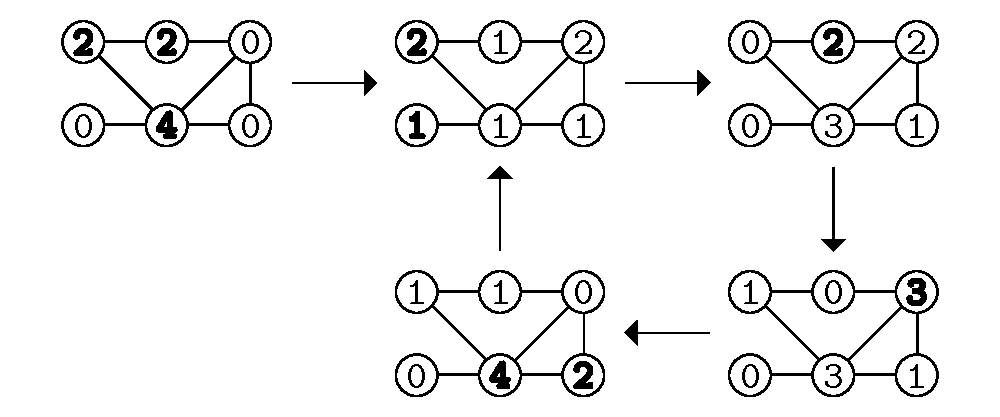
\includegraphics[width=\figWidthA]{Figures/example}}
\subfloat{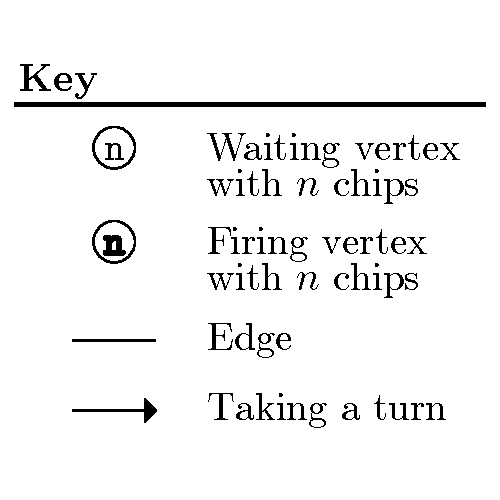
\includegraphics[width=\figWidthB]{Figures/keyShort}}
\caption{A parallel chip-firing game. From an initial position in the upper
  left, the game eventually enters a period of length 4.}
\label{example}
\end{figure}

The total number of chips on all vertices of the graph is constant throughout a
game, so there are finitely many possible positions in every game. Therefore,
every game eventually reaches a position $\pos{t}$ that is identical to a later
position $\pos{t+p}$ for some $t,p \in \nats$ with $p > 0$. (We write $\pos{t}
= \pos{t+p}$.) The game is deterministic, so $\pos{t+n} = \pos{t+n+p}$ for all
$n \in \nats$. Thus, every parallel chip-firing game is eventually periodic.

In this paper, we concern ourselves with both \emph{firing sequences} and
\emph{periodic firing patterns} of vertices. Each is a binary string
representing whether or not a particular vertex fires or waits each turn. The
sequence covers all times from 0 to infinity, while the periodic pattern covers
just one period.

\subsection*{Previous Work}
The periodicity of the parallel chip-firing game gives rise to two
questions. First, what characteristics of a game and its underlying graph
determine the length of a period? It is known exactly what periods are possible
on certain classes of graphs, such as trees~\cite{bitarGoles}, simple
cycles~\cite{cycle}, the complete graph~\cite{levine}, and the complete
bipartite graph~\cite{jiang}. Kiwi et al.~\cite{kiwiEtAl} constructed graphs on
which the period of games can grow exponentially with polynomial increase in
the number of vertices. There are also results regarding the total number of
chips in a game. Kominers and Kominers~\cite{kominers} showed that games with a
sufficiently large density of chips must have period~1. Dall'Asta~\cite{cycle}
and Levine~\cite{levine}, in their respective characterizations of periods on
cycles and complete graphs, related the total number of chips to a game's
\emph{activity}, the fraction of turns during which a vertex fires. The
denominator of the activitymust divide the period.

Second, we notice that some but not all positions $\pos{t}$ are
\emph{periodic}, satisfying $\pos{t} = \pos{t+p}$ for some positive $p \in
\nats$. What characterizes periodic positions? This problem has not been as
extensively studied. Dall'Asta~\cite{cycle} characterized the periodic
positions of games on cycles.

\subsection*{Our Results}
We hope to advance the understanding of both of these questions through the
study of firing sequences and periodic firing patterns.

After precisely defining the parallel chip-firing game in Section~\ref{pres},
the first half of the paper develops a new tool for studying the chip-firing
game: \emph{motors}, vertices that fire with a regular pattern independent of
normal chip-firing rules. Games with motors are called \emph{motorized
  games}. Motors allow us to study the behavior of subgraphs in ordinary
parallel chip-firing games. In Section~\ref{motors} we show that vertices
always ``follow'' a motor in periodic motorized games on trees. In
Section~\ref{simulatingMotors}, we prove that periodic motorized games can be
transformed into ordinary games as long as the firing sequence of each motor
occurs in an ordinary game.

The second half of the paper characterizes the possible periodic firing
patterns in parallel chip-firing games. Section~\ref{binSeq} briefly steps away
from the game to study certain signed sums of periodic binary sequences. The
result is an inequality applicable to edges of the graph of a parallel
chip-firing game. In Section~\ref{nonclumpiness}, we sum this inequality over
all relevant edges to show that periodic firing patterns with both consecutive
0s and consecutive 1s cannot occur in a parallel chip-firing game. This, along
with an already known construction, fully characterizes the periodic firing
patterns possible in parallel chip-firing games. Finally, in
Section~\ref{corollaries}, we examine some implications of this theorem.
